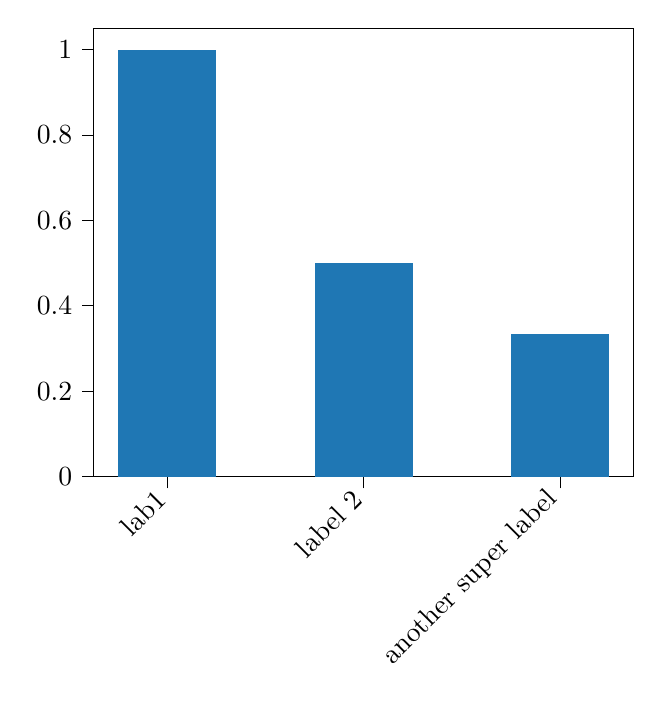
\begin{tikzpicture}

\definecolor{darkgray176}{RGB}{176,176,176}
\definecolor{steelblue31119180}{RGB}{31,119,180}

\begin{axis}[
tick align=outside,
tick pos=left,
x grid style={darkgray176},
xmin=-0.375, xmax=2.375,
xtick style={color=black},
xtick={0,1,2},
xticklabel style={rotate=45.0,anchor=east},
xticklabels={lab1,label 2,another super label},
y grid style={darkgray176},
ymin=0, ymax=1.05,
ytick style={color=black}
]
\draw[draw=none,fill=steelblue31119180] (axis cs:-0.25,0) rectangle (axis cs:0.25,1);
\draw[draw=none,fill=steelblue31119180] (axis cs:0.75,0) rectangle (axis cs:1.25,0.5);
\draw[draw=none,fill=steelblue31119180] (axis cs:1.75,0) rectangle (axis cs:2.25,0.33333333);
\end{axis}

\end{tikzpicture}
